\documentclass{beamer}

\usepackage[utf8]{inputenc}

\input{../../helper}
\graphicspath{{img/}}

\title{Introdução à Computação \\ Laboratório 1}
\author{Alexandre Rademaker}
\date{}

\begin{document}

\begin{frame}
 \maketitle
\end{frame}

\begin{frame}[allowframebreaks,fragile]{linha de comando}

  Muitos sistemas operacionais modernos têm interfaces gráficas de
  usuário (GUI) para permitir fácil navegação e manipulação de
  arquivos e pastas com o mouse.

  Ainda assim, como programador, você provavelmente usará a janela do
  terminal com frequência e poderá realizar muitas das mesmas tarefas
  através de comandos.

  Estes comandos podem ser repetidos e até podemos programar
  \emph{scripts}.

  \framebreak

  Vamos ver alguns comandos mais comuns no sistemas Linux e MacOS. No
  Windows também podem ser encontrados no
  \href{https://en.wikipedia.org/wiki/Windows_Subsystem_for_Linux}{WSL}.

  O comando \ilcode{ls} lista os arquivos de uma pasta.

  O comando \ilcode{cd} muda o diretório (pasta) corrente. Os símbolos
  \ilcode{.} e \ilcode{..} correspondem ao diretório corrente e ao
  diretório pai do corrente. Diretórios podem ser relativos ou
  absolutos.\vspace{.5cm}

  \begin{lstlisting}[style=normalbash]
    cd ..
    cd ../dir1/dir2/dir3
  \end{lstlisting}

  \framebreak

  Podemos criar diretórios como o \ilcode{mkdir}.

  Podemos copiar arquivos e diretórios com o \ilcode{cp}. Também
  podemos fazer cópias recursivas com a opção \ilcode{-r}.

  Podemos remover arquivos com \ilcode{rm}, evitando confirmação com a
  opção \ilcode{-f} e para remover diretórios precisamos passar
  \ilcode{-r}. E podemos passar os argumentos juntos com \ilcode{-rf}.

  Podemos mover arquivos com \ilcode{mv} que também recebe origem e
  destino como parâmetros, podendo ser diretórios ou arquivos.

  \framebreak

  Existem vários outros como: \ilcode{touch}, \ilcode{diff},
  \ilcode{rmdir}, \ilcode{clear}, \ilcode{chmod} etc.

  Use \ilcode{man CMD} para obter o manual do comando \ilcode{CMD},
  por exemplo, \ilcode{man ls}.
  
\end{frame}

\begin{frame}[allowframebreaks,fragile]{tipos de dados}

  Uma \emph{constante} ou \emph{variábel} é basicamente um local
  nomeado da memória que contém um valor durante a execução do
  programa.

  Os \emph{literais} são os valores que atribuímos às variáveis ou
  constantes.

  Geralmente, podemos usar os termos literal e constante de forma
  intercambiável. Por exemplo, na expressão \ilcode{const int a = 7;}
  declaramos o nome \ilcode{a} como uma constante do tipo \ilcode{int}
  enquanto nos referimos ao valor 7 como um literal do tipo inteiro.

  Os literais \ilcode{3.4} ou \ilcode{3.4E4} são valores do tipo
  ponto-flutuante. E o literal \ilcode{'a'} é um caracter.

  \framebreak

  O tipo \ilcode{int} é usado para armazenar inteiros.

  Inteiros sempre ocupam 4 bytes de memória (32 bits). Isso significa
  que o intervalo de valores que eles podem armazenar é
  necessariamente limitado a 32 bits de informação.

  \begin{center}
    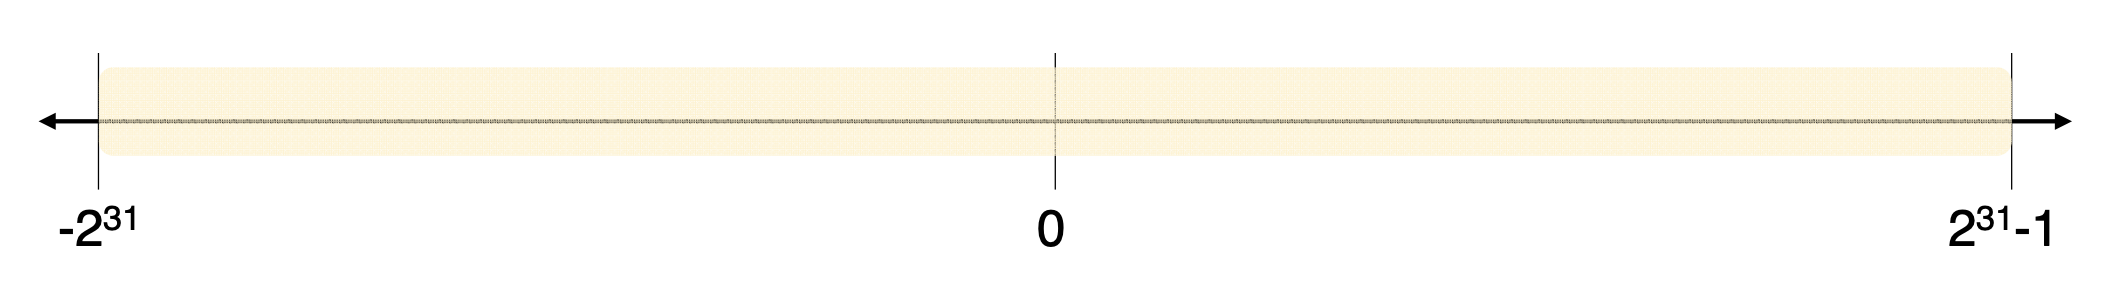
\includegraphics[width=.8\textwidth]{int.png}
  \end{center}

  \framebreak

  \ilcode{unsigned} é um \emph{qualificador} que pode ser aplicado a
  certos tipos (incluindo \ilcode{int}), o que efetivamente dobra o
  intervalo positivo desse tipo, ao custo de não permitir valores
  negativos. \vspace{.5cm}

  \begin{lstlisting}[style=normalc]
    unsigned int a = 100;
  \end{lstlisting}

  \begin{center}
    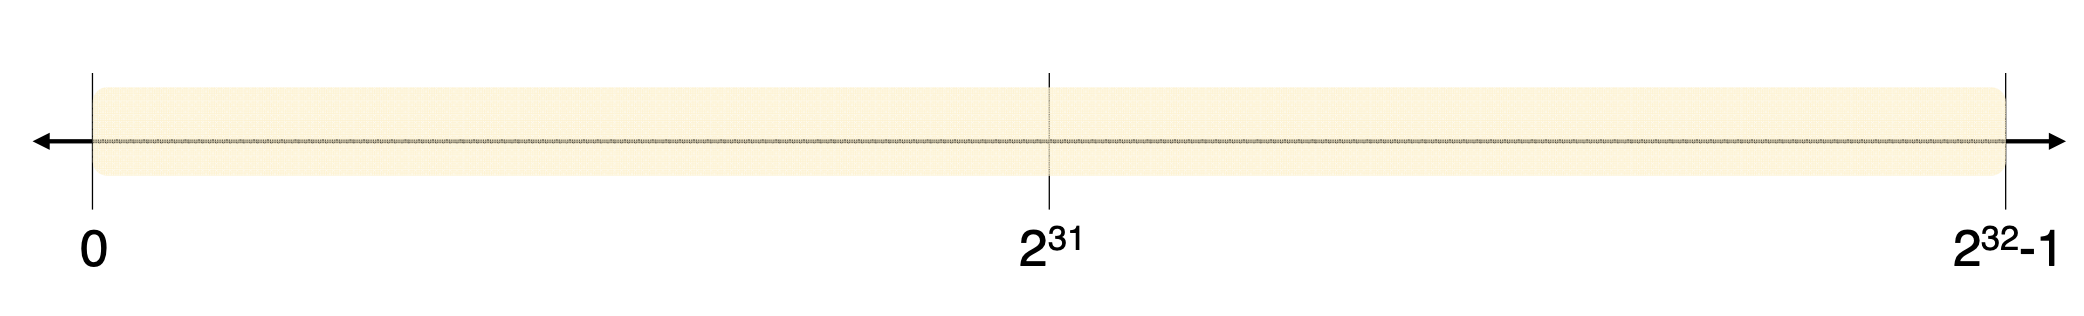
\includegraphics[width=.8\textwidth]{unsigned-int.png}
  \end{center}

  \framebreak

  O tipo de dados \ilcode{char} é usado para variáveis que armazenam
  caracteres.

  Os caracteres sempre ocupam 1 byte de memória (8 bits). O intervalo
  de valores que eles podem armazenar é necessariamente limitado a 8
  bits de informação.

  A tabela ASCII, oferece um mapeamento de caracteres como A, a, B, C,
  etc... para valores numéricos no lado positivo deste intervalo.

  \begin{center}
    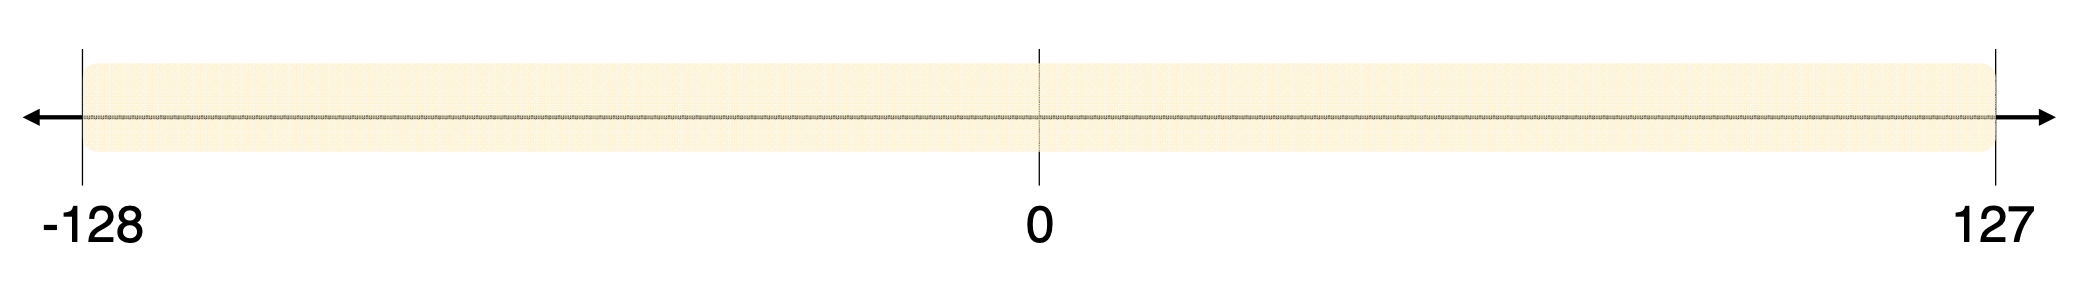
\includegraphics[width=.8\textwidth]{char.png}
  \end{center}

  \framebreak

  O tipo de dados \ilcode{float} é usado para variáveis que irão
  armazenar valores de ponto flutuante, números reais.

  Valores de pontos flutuantes sempre ocupam 4 bytes de memória (32
  bits).

  Com 32 bits de precisão, alguns dos quais podem ser usados para uma
  parte inteira, estamos limitados em quão precisos podemos ser. Mais
  \href{https://learn.microsoft.com/en-us/cpp/c-language/c-floating-point-constants?view=msvc-170}{aqui}.

  \framebreak

  O tipo de dados \ilcode{double} é usado para variáveis que irão
  também armazenar valores de ponto flutuante. A diferença é que
  doubles são precisão dupla. Eles ocupam sempre 8 bytes de memória
  (64 bits).

  Com 32 bits adicionais de precisão em relação a um \ilcode{float},
  os doubles nos permitem especificar números reais muito mais
  precisos.

  \framebreak

  O tipo \ilcode{void} é um tipo, mas não um tipo de dados.
  
  As funções podem ter um tipo de retorno \ilcode{void}, o que
  significa apenas que não retornam um valor.

  A lista de parâmetros de uma função também pode ser
  \ilcode{void}. Significa simplesmente que a função não aceita
  parâmetros. Um substituto para `nada'.

  \framebreak

  O tipo \ilcode{bool} contém apenas dois valores: \ilcode{true} e
  \ilcode{false}.

  Para usar estas constantes, devemos importar a biblioteca
  \ilcode{stdbool.h} com a macro \ilcode{#include <stdbool.h>}.

  \framebreak

  Também encontraremos estruturas (\ilcode{structs}) e tipos definidos
  (\ilcode{typedef}) que oferecem grande flexibilidade na criação dos
  tipos de dados necessários para seus programas.
  
\end{frame}


\begin{frame}[allowframebreaks,fragile]{Variáveis}

  C exige que você especifique o tipo de dados de cada variável, na
  criação da variável com ou sem sua inicialização.

  Variáveis podem ser declaradas sem serem inicializadas. 

  \begin{lstlisting}[style=normalc]
    int a = 10; 

    int a;    
    a = 10;   
  \end{lstlisting}

  \framebreak

  Se você deseja criar várias variáveis do mesmo tipo, especifique o
  nome do tipo uma vez e, em seguida, liste quantas variáveis desse
  tipo desejar.

  \begin{lstlisting}[style=normalc]
    int height, width;
    float sqrt2, sqrt3, pi;
  \end{lstlisting}
  
  Em geral, é recomendável declarar variáveis apenas quando necessário.

\end{frame}


\begin{frame}[allowframebreaks,fragile]{Operadores}

  Para manipular variáveis e valores em C, precisamos de
  operadores. Os operadores permitem construir valores a partir de
  outros valores.

  Em C temos a adição (\ilcode{+}), subtração (\ilcode{-}),
  multiplicação (\ilcode{*}) e divisão (\ilcode{/}) de números,
  \emph{operadores aritméticos}. Também temos o módulo (resto da
  divisão, \ilcode{\%}). \vspace{.5cm}

  \begin{lstlisting}[style=normalc]
    int x = y + 1;
    x = x * 5;
    int m = 13 % 4;
  \end{lstlisting}

  \framebreak

  Também podemos usar algumas formas abreviadas (açucares sintáticos)
  para combinar expressões com a atualização de valores em variáveis.\vspace{.5cm}

  \begin{lstlisting}[style=normalc]
    x = x * 5;
    x *= 5;

    x = x + 1;
    x++;
    
    x = x - 1;
    x--;
  \end{lstlisting}

  \framebreak

  Expressões booleanas são usadas em C para comparar valores.
  
  Todas as expressões booleanas em C são avaliadas como um dos dois
  valores booleanos possíveis – verdadeiro ou falso.
  
  Podemos usar o resultado da avaliação de uma expressão booleana em
  outras construções de programação, como condicionais.

  \framebreak

  Às vezes, ao trabalhar com expressões booleanas, usaremos variáveis
  do tipo bool, mas nem sempre.
  
  Em C, todo valor diferente de zero é equivalente a \ilcode{true} e
  zero é \ilcode{false}.

  Expressões booleanas são construídas com operadores lógicos e
  operadores relacionais.

  \framebreak

  O AND lógico (\ilcode{\&\&}) é verdadeiro se e somente se ambos os
  operandos forem verdadeiros, caso contrário, falso.

  \begin{center}
    \begin{tabular}{ccc}
      x & y & x \&\& y\\
      \hline
      true & true & true\\
      true & false & false\\
      false & true & false\\
      false & false & false\\ \hline
    \end{tabular}
  \end{center}

  \framebreak

  O OR lógico (\ilcode{\|\|}) é verdadeiro se e somente se pelo menos um
  operando for verdadeiro, caso contrário, falso.

  \begin{center}
    \begin{tabular}{ccc}
      x & y & x \verb#||# y\\
      \hline
      true & true & true\\
      true & false & true\\
      false & true & true\\
      false & false & false\\ \hline
    \end{tabular}
  \end{center}

  O NOT lógico (\ilcode{!}) inverte o valor de seu operando.

  \framebreak

  Os operadores relacionais se comportam como você esperaria e parecem
  sintaticamente semelhantes a como você pode recuperá-los da
  aritmética elementar.

  \begin{itemize}
  \item Less than (\ilcode{x < y})
  \item Less than or equal to (\ilcode{x <= y})
  \item Greater than (\ilcode{x > y})
  \item Greater than or equal to (\ilcode{x >= y})
  \end{itemize}

  \framebreak

  Também podemos testar igualdade (\ilcode{x == y}) ou desigualdade
  (\ilcode{x != y}).

  {\color{red} Cuidado}! É um erro comum usar o operador de atribuição
  (\ilcode{=}) quando você pretende usar o operador de igualdade
  (\ilcode{==}).
  
\end{frame}

\begin{frame}[allowframebreaks,fragile]{Condicionais}

  As expressões condicionais permitem que seus programas tomem
  decisões e façam diferentes bifurcações no fluxo de execução,
  dependendo de testes lógicos.
  
  C fornece algumas construções diferentes para implementar
  condicionais.

  \begin{lstlisting}[style=normalc]
    if (boolean-expression) {
      // code
    }
  \end{lstlisting}

  \framebreak

  Também podemos especificar um bloco para ser executado caso a
  expressão booleana seja falsa.

  \begin{lstlisting}[style=normalc]
    if (boolean-expression) {
      // code
    }
    else {
      // code
    }
  \end{lstlisting}

  \framebreak

  E podemos criar uma cadeia de testes mutuamente exclusivos.

  \begin{lstlisting}[style=normalc]
    if (boolean-expression1) {
      // code
    }
    else if (boolean-expression2) {
      // code
    }
    else if (boolean-expression3) {
      // code
    }
    else {
      // code
    }
  \end{lstlisting}

  \framebreak

  Ou não mutuamente exclusivos.

  \begin{lstlisting}[style=normalc]
    if (boolean-expression1) {
      // code
    }
    if (boolean-expression2) {
      // code
    }
    if (boolean-expression3) {
      // code
    }
    else {
      // code
    }
  \end{lstlisting}

  \framebreak

  Também temos o operador \ilcode{switch} que permite enumerar casos
  para uma data expressão. Observe os \ilcode{break}.

  \begin{lstlisting}[style=normalc]
    int x = <valor>;
    switch(x) {
      case 1:
       printf("one!");
       break;
      case 2:
       printf("Two!");
       break;
      case 3:
       printf("Three!");
       break;
      default:
       printf("Sorry!");
    }
  \end{lstlisting}

  \framebreak

  Finalmente, também podemos escrever uma expressão com o operador
  ternário \ilcode{?:}. Note que blocos de apenas uma instrução não
  precisam das chaves.\vspace{.5cm}

  \begin{lstlisting}[style=normalc]
    int x = (bool-expr) ? 5 : 6;

    int x;
    if (bool-expr) 
      x = 5;
    else
      x = 6;
  \end{lstlisting}
\end{frame}

\begin{frame}[allowframebreaks,fragile]{Loops ou repetições}

  \begin{description}
  \item[while] use quando quiser que um loop seja repetido um número
    desconhecido de vezes e, eventualmente, nenhuma.
  \item[do-while] use quando quiser que um loop seja repetido um
    número desconhecido de vezes, mas pelo menos uma vez.
  \item[for] use quando quiser que um loop se repita um número
    discreto de vezes, embora você possa não saber o número no momento
    em que o programa é compilado.
  \end{description}

  \framebreak

  Ao encontrar o comando \ilcode{for}, o programa irá executar o
  comando \ilcode{start}. A expressão \ilcode{expr} é avaliada. Se for
  verdadeira, o bloco é executado. Se for falsa, o bloco não é
  executado e o fluxo passa para o próximo comando depois do
  \ilcode{for}. Se o bloco for executado, após ele, o comando
  \ilcode{increment} é executado e novamente \ilcode{expr} é avaliada
  e o ciclo continua.\vspace{.5cm}

  \begin{lstlisting}[style=normalc]
    for (start; expr; increment) {
      // code
    }
  \end{lstlisting}

  \framebreak

  No primeiro caso o bloco pode não ser executado nenhuma vez. No
  segundo, pelo menos a primeira vez ele será executado.\vspace{.5cm}

  \begin{lstlisting}[style=normalc]
    while (boolean-expr) {
      // code
    }

    do {
      // code
    } while (boolean-expr)
  \end{lstlisting}

\end{frame}

\begin{frame}[allowframebreaks,fragile]{números mágicos}

  Constantes em nosso código às vezes são chamadas de números mágicos.

  Imagine que seu código depende de certas constantes que, a
  princípio, você não pensa em mudar. Eventualmente, este número
  poderá ter que ser usado em mais de um local.

  Imagine que em algum momento no futuro, você precisa alterar este
  valor. Agora terá que procurar em todos os trechos do código para
  não introduzir um \emph{bug}.

  \framebreak

  Imagine um programa manipulando cartas de um baralho. Outras funções
  deste programa provavelmente também precisarão da constante 52.

  \begin{lstlisting}[style=normalc]
    card deal_cards(deck name) {
      for (int i = 0; i < 52; i++) {
        // deal the card
      }
    }
  \end{lstlisting}

  \framebreak

  Podemos usar uma \emph{macro} para que o pré-processador (antes do
  compilador) substitua ocorrências de um nome pela expressão
  associada.

  Se \ilcode{#include} é como copiar/colar, o \ilcode{#define} é
  análogo ao find/replace.\vspace{.5cm}

  \begin{lstlisting}[style=normalc]
    #define DECKSIZE 52

    card deal_cards(deck name) {
      for (int i = 0; i < DECKSIZE; i++) {
        // code
      }
    }
  \end{lstlisting}

  \framebreak

  Um outro exemplo bem prático é para definir constantes que possamos
  precisar em várias partes do programa.\vspace{.5cm}

  \begin{lstlisting}[style=normalc]
    #define PI 3.14159265    
  \end{lstlisting}

  Geralmente declaramos estas diretivas no topo dos arquivos
  \ilcode{.c} e geralmente usamos nomes em maiúsculas.

\end{frame}

\end{document}


%%% Local Variables:
%%% mode: latex
%%% TeX-master: t
%%% End:
